
\documentclass[11pt,a4paper]{article}
\usepackage[left=2cm,right=2cm,top=2cm,bottom=3cm]{geometry}
\usepackage{amsmath,amsfonts,amsthm,amssymb,varioref,times, commath}
\usepackage{gensymb}
\usepackage{tikz}
\usepackage{textcomp}
\usepackage{hyperref}
\hypersetup{
 colorlinks=true,
 linkcolor=blue,
 filecolor=magenta, 
urlcolor=cyan,
}
\usepackage{lipsum}
\usepackage{epigraph}
%to resume numbering in a list
\usepackage{enumitem}
%----- arrows 
\usepackage{extarrows}

%    differential equatiosn 
\usepackage{diffcoeff}   %\diff[2]{x}{y}


%%%%%%pour ecrire en français avec les accents
\usepackage[utf8]{inputenc}
\usepackage[T1]{fontenc}
\usepackage{lmodern} % load a font with all the characters
\usepackage{units}
%%%%%%%Image-related packages
\usepackage{wrapfig}
\usepackage{float, graphicx}
\graphicspath{ {./img/} }
\usepackage{subcaption}
\usepackage[export]{adjustbox}

%%%%%%%pour faire des cadres
\usepackage{xcolor}
\usepackage{tcolorbox}
\usepackage{framed}
\usepackage{mdframed}


%%%%%%%chemistry frmulae
\usepackage{chemfig}
\usepackage{chemformula}
\usepackage[version=4]{mhchem}

% -------------- Circuits -------------------
\usepackage[european, straightvoltages]{circuitikz}

% Title & headers
\usepackage[explicit]{titlesec}
% Raised Rule Command:
% Arg 1 (Optional) - How high to raise the rule
% Arg 2 - Thickness of the rule
\newcommand{\raisedrulefill}[2][0ex]{\leaders\hbox{\rule[#1]{1pt}{#2}}\hfill}
\titleformat{\section}{\Large\bfseries}{\thesection. }{0em}{#1\,\raisedrulefill[0.4ex]{1pt}}

% pour ecrire sur +sieurs colonnes
\usepackage{multicol}
\setlength{\columnseprule}{0pt}
\setlength{\columnsep}{60pt}
% Fusion de lignes de tableaux.
\usepackage{multirow}
% Position verticale des lettres dans la ligne de tableau.
\usepackage{array}

% physics -----------------------------------------------------------
\newcommand{\To}{\longrightarrow}
\newcommand{\gpl}{\; g\cdot L^{-1}}
\newcommand{\gpmol}{\; g\cdot mol^{-1}}
\newcommand{\mpl}{\; mol\cdot L^{-1}}
\newcommand{\mps}{\; m\cdot s^{-1}}
\newcommand{\rps}{\; rad\cdot s^{-1}}
\newcommand{\kph}{\; km\cdot h^{-1}}
\newcommand{\mpss}{\; m\cdot s^{-2}}
\newcommand{\Dt}{\Delta t}
\newcommand{\vv}{\vec{v}}
\newcommand{\va}{\vec{a}}
\newcommand{\vp}{\vec{p}}
\newcommand{\vf}{\vec{F}}
\newcommand*{\Vf}[1]{\overrightarrow{F_\ensuremath{{#1}}}}
\newcommand{\es}[1]{\cdot10^{#1}}
\newcommand{\eng}[1]{\textcolor{purple}{(= #1})}
\usepackage{harpoon}
%\newcommand*{\vect}[1]{\overrightharp{\ensuremath{#1}}}
\newcommand*{\Vect}[1]{\overrightarrow{\ensuremath{#1}}}
\newcommand{\pfd}[1]{\sum \vec{F}_{ext_{#1}} &= \od{\vp_{#1}}{t} = m\cdot\va_{#1}}
\newcommand{\C}{\degree C}
\newcommand{\Delt}{\Delta t}

% --- Circuits ------------
\newcommand{\bipole}[1]{
\begin{circuitikz} \draw
(0,0) to[ #1 ] (2,0); 
\end{circuitikz} {\hspace{5mm}}}

% Chimie ---------------------------------
\newcommand{\oxo}{\ce{H3O+}_{(aq)}}
\newcommand{\eau}{\ce{H2O}_{(\ell)}}
\newcommand{\OH}{\ce{HO-}_{(aq)}}
\newcommand{\AH}{\ce{AH}_{(aq)}}
\newcommand{\A}{\ce{A-}_{(aq)}}
\newcommand{\MnO}{\ce{MnO_4^{-}}}
\newcommand{\conc}[1]{\left[{#1}\right]}
\newcommand{\couple}[2]{\ce{#1/#2}}


% Environnements ------------------------
\newcounter{exo}
\newenvironment{exo}[1][]
{\refstepcounter{exo} \begin{shaded}\noindent $\triangleright \quad$\textbf{Exercice~\theexo. #1} } { \end{shaded}}
\newenvironment{eg}
{\begin{shaded} \textbf{Exemple:} } { \end{shaded}}

\newenvironment{defn}[1]
{\begin{leftbar}\noindent \textbf{Définition :\textit{ \quad #1}} } { \end{leftbar}}

%\newenvironment{rmrq}
%{\begin{shaded} \textbf{Remarque.\quad } \itshape } { \end{shaded}}
\newenvironment{rmrq}
{\begin{mdframed}[backgroundcolor=blue!10, linewidth=0pt] \textbf{Remarque.\quad } \itshape } { \end{mdframed}}

\newenvironment{python}
{\begin{shaded} \textbf{A faire en PYTHON}\\ \itshape } { \end{shaded}}

% Shading colour -----------------------------
\definecolor{shadecolor}{gray}{0.9}

\date{}
\author{}

\renewcommand*\contentsname{Résumé}









% Title & headers 
\usepackage{fancyhdr}
\pagestyle{fancy}
\fancyhf{}
\lhead{SciPhy : Terminale spé}
\rhead{$\Phi $ - 6 : Lunettes astronomiques}
\chead{2020-28}
\rfoot{Page \thepage}
\lfoot{\textcopyright\; S Zayyani}
\renewcommand{\footrulewidth}{0.1pt}% default is 0pt

\title{\large Physique - Chapitre 6 \\ \LARGE  La lunette astronomique}
\date{}
\author{}

\setlength{\parindent}{0mm}
\setlength{\parskip}{2mm}

%%%%%%%%%%% For wrapfigure 
\setlength{\intextsep}{6pt}%
\setlength{\columnsep}{3pt}%

\def\width{17}
\def\hauteur{5}

\begin{document}
\maketitle
\vspace{-1cm}
\begin{tcolorbox}[title=Notions de la classe de première à rappeler]
les bases de l'optique géométrique ; lentilles minces ; tracer un rayon lumineux à travers une lentille
%\tcblower
\end{tcolorbox}
\tableofcontents

\section{Rappels}

\subsection{Voir un objet}

Pour que l’on puisse voir un objet, il faut réunir certaines conditions, notamment que l’œil «détecte» la présence de l’objet.  

Ceci entraîne l’arrivée de la lumière provenant de l’objet dans l'\oe il. Il faut donc, dans un premier temps, que l’objet émette de la lumière. Cette lumière pourrait être produite par l’objet, et dans ce cas-là l’objet est une \textbf{source primaire de lumière} (objet lumineux) ; ou la lumière pourrait être diffusée par l’objet, et dans ce cas l’objet est une \textbf{source secondaire} de lumière (objet éclairé). 

Mais dans un deuxième temps, il faut des conditions propices au passage de la lumière de l’objet vers l’œil humain, c’est-à-dire des conditions nécessaires pour la propagation de la lumière.  

Une source lumineuse ponctuelle émet de la lumière dans tous les sens. L'ensemble des rayons lumineux qui pénètrent dans l’œil forment un \textbf{faisceau lumineux}. Quand la source lumineuse s’éloigne, l’angle du faisceau lumineux se rapproche de 0\degree. Pour un objet situé très loin, on dit qu'il se situe « à l’infini », et les rayons pénétrant l’œil sont considérés comme \textbf{parallèles}. 

\subsection{Lentilles}

De manière générale une lentille \eng{lens} est un système optique qui sert à dévier et à déformer un faisceau\eng{beam} de lumière. La lentille la plus simple est un objet transparent avec une surface courbée. Elles le fait grâce à la réfraction du faisceau lumineux pendant l'entrée (et souvent la sortie) du faisceau dans le système optique. Comme nous allons voir par la suite, il y a différentes catégories de lentilles. Celles qui nous intéressent et que l'on va étudier sont des lentilles minces. 

\subsection{Lentilles minces}

\begin{defn}{Lentilles minces}
\begin{itemize}
    \item Une lentille mince est une lentille dont l’épaisseur reste faible devant les rayons de courbure de ses faces.
    \item Il existe deux catégories de lentilles, des lentilles convergentes : 
    \begin{itemize}
        \item Les lentilles \textbf{convergentes} sont plus épaisses au centre qu’au bord.  Elles font converger le faisceau lumineux qui les traverse (cf. 1, 2, 3 dans la figure \ref{fig:lentillemince}.)
        \item Les lentilles \textbf{divergentes} sont plus épaisses au bord qu’au centre.  Elles font diverger le faisceau lumineux qui les traverse (cf. 3, 4, 5 dans la figure \ref{fig:lentillemince}). 
    \end{itemize}
\end{itemize}
\end{defn}

\begin{figure}[h]
    \centering
    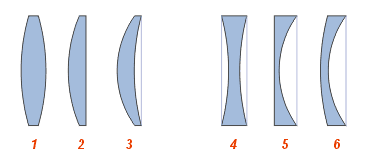
\includegraphics[width=0.7\linewidth]{imgs/p6/lentilles minces.png}
    \caption{exemples de lentilles minces}
    \label{fig:lentillemince}
\end{figure}

\subsection{Caractérisation d'une système optique}

\begin{figure}[h]
    \centering
\begin{tikzpicture}[scale=1,decoration={markings,mark=at position 1cm with {\arrow[]{stealth};}}] 
\coordinate (O1) at (0,0);%centre optique de la première lentille
\coordinate (A) at (-5,0);%position de l'objet
\coordinate (B) at (-5,1);%sommet de l'objet
\def \focaleUn{2};%focale de la première lentille
\coordinate (A') at (3.33,0);%position de l'objet
\coordinate (B') at (3.33,-0.667);%sommet de l'objet
%\draw[help lines] (-7,-3) grid (7,3);
%\draw[very thin, lightgray, step=2mm] (-7,-3) grid (7,3);
\draw[thin,->](-5,0)--++(10,0)node[above right,fill=white]{\tiny +};
%\draw[|->, thick] (A)node[below]{A}--(B)node[above]{B};
%\draw[|->, thick,gray] (A')node[above]{A'}--(B')node[below]{B'};
\draw[shift={(O1)},ultra thick,<->,>=latex] (0,-2)--++(0,4) node[above]{$\mathcal{L}$};%lentille convergente
%\draw[shift={(B)},red, postaction={decorate},->] (0,0)--++(5,0)--++({-atan(1/2)}:5);
%\draw[shift={(B)},red, postaction={decorate},->] (0,0)--++({-atan(1/5)}:11);
%\draw[shift={(B)},red, postaction={decorate},->] (0,0)--++({-atan(1/3)}:5.27)--++(5,0);
\foreach \x/\z in {O1/\focaleUn}{
\draw[shift={(\x)}] (0,0) node[below left] {O};
\draw[shift={(\x)}] (\z,2pt) --++ (0,-4pt) node[below] {F'};
\draw[thin, dotted] (-2,-2) -- (-2,2) ; 
\draw[thin, dotted] (2,-2) -- (2,2) ; 
\draw[shift={(\x)}] ({-\z},2pt) --++ (0,-4pt) node[below] {F};
}
\end{tikzpicture}
\caption{Un système optique}
\label{fig:système optique}
\end{figure}

Les lentilles minces sont caractérisées par : 
\begin{itemize}
    \item \textbf{Centre optique (O) : }le point particulier où un rayon incident n’est pas dévié. 
    \item \textbf{Foyer image ($F’$) \eng{focal point}:} le point de convergence des rayons lumineux arrivant de l’infini (i.e. parallèles).
    \item \textbf{Plan focal image \eng{focal plane}: } on appelle plan focal image le plan perpendiculaire à l'axe optique passant par le foyer image $F'$.
	\item \textbf{Foyer objet ($F$) :} le point dont l’image se trouve à l’infini après avoir traversé la lentille. Il est situé à la même distance que le foyer image, par rapport au centre optique, mais de l’autre côté de la lentille. 
	\item \textbf{Plan focal objet : }on appelle plan focal objet le plan perpendiculaire à l'axe optique passant par le foyer objet $F$.
	\item \textbf{Distance focale ($f’$) \eng{focal length}:} la distance entre le foyer image et le centre optique. ($\overline{OF'}=f'$) et ($\overline{OF}=f$). 
	\item \textbf{Vergence (C) :} Inverse de la distance focale. $C=\dfrac{1}{f'}$  .  La vergence s’exprime en « \textit{dioptries} » dont le symbole est $\delta$ (quand $f'$ est exprimé en \textit{mètres}). 
\end{itemize}
\begin{rmrq}
\textbf{Remarque :} la barre sur $OF$ signifie une \emph{grandeur orientée}. c'est-à-dire $\overline{OF'}=f'=-\overline{OF}=-f$ et $OF'=OF$. 
\end{rmrq}

\subsection{Construire l'image d'un objet}

Mettons en place maintenant les règles pour la construction graphique de l’image d’un objet donnée par une lentille mince.  En général si on prend un point B sur l’objet, on peut trouver son image en suivant les règles suivantes :
\begin{itemize}
    \item \textcolor{blue}{Un rayon lumineux passant par $O$ n’est jamais dévié}.
    \item \textcolor{red}{Un rayon arrivant, qui est parallèle à l’axe optique, émerge en passant par le foyer image $F'$.} 
    \item \color{Green}{Un rayon arrivant, en passant par le foyer objet $F$, émerge parallèle à l’axe optique.}  
\end{itemize}

\begin{figure}[H]
    \centering
    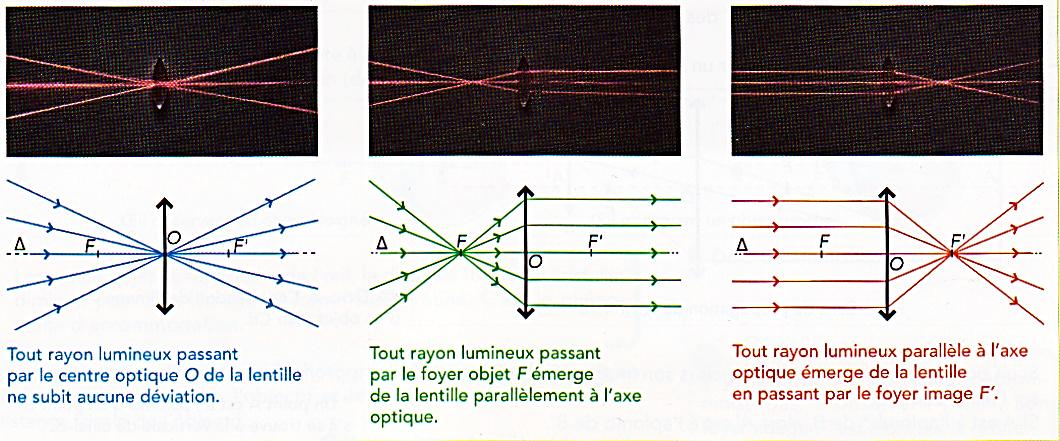
\includegraphics[width=\textwidth]{imgs/p6/rayons.jpg}
    \caption{Comportement des rayons à travers une lentille convergente.}
    \label{fig:rayonsconvergent}
\end{figure}

Les lentilles minces \textbf{convergente} et \textbf{divergente} sont identiques avec la seule différence étant l'inversion des foyers objets et image: dans une lentille convergente le foyer image se situe après le centre optique, tandis que pour une lentille divergente le foyer image se situe avant le centre optique (cf. \ref{fig:convergediverge} )

\begin{figure}[ht]
\centering
\begin{subfigure}{.47\textwidth}
  \centering
  % include first image
  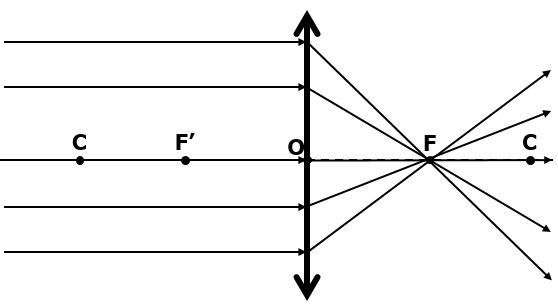
\includegraphics[width=.95\linewidth]{imgs/p6/convergente.jpg}  
\end{subfigure}
\begin{subfigure}{.47\textwidth}
  \centering
  % include first image
  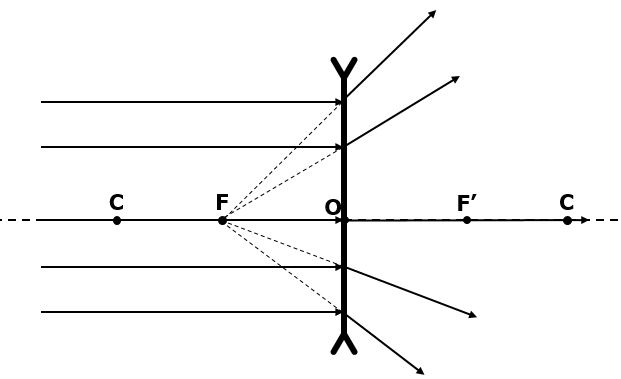
\includegraphics[width=.95\linewidth]{imgs/p6/divergente.jpg}  
\end{subfigure}
\caption{Lentille convergente à gauche \& lentille divergente à droite.}
\label{fig:convergediverge}
\end{figure}


Nous représentons normalement un objet par une \textbf{flèche verticale} ($AB$), perpendiculaire à l’axe optique.  \textbf{En traçant au moins deux de ces trois rayons}, le point $B’$ (image du point $B$) est situé à l’intersection des rayons émergents, comme détaillé dans les figures suivantes : 

\begin{figure}[ht]
\centering
\begin{subfigure}{.18\textwidth}
  \centering
  % first image
  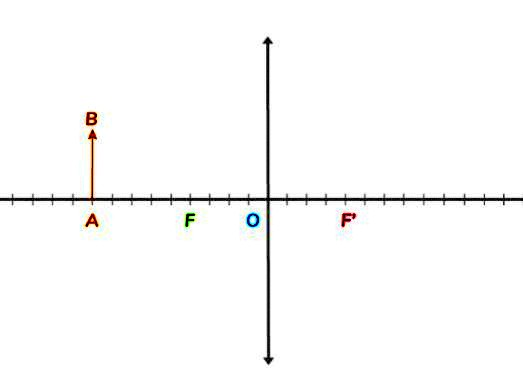
\includegraphics[width=.95\linewidth]{imgs/p6/construct1.jpg}  
\end{subfigure}
\begin{subfigure}{.18\textwidth}
  \centering
  % second image
  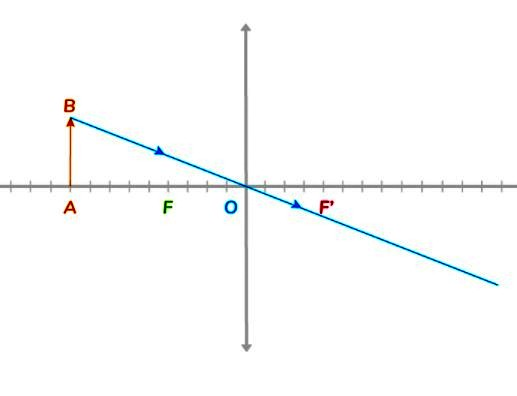
\includegraphics[width=.95\linewidth]{imgs/p6/constrcut2.jpg}  
\end{subfigure}
\begin{subfigure}{.18\textwidth}
  \centering
  % third image
  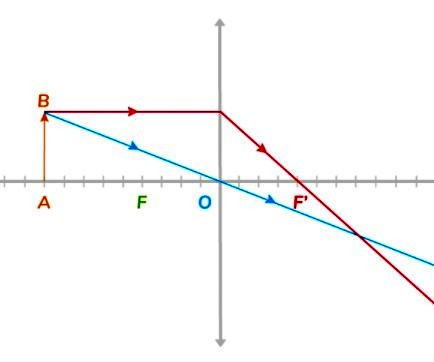
\includegraphics[width=.95\linewidth]{imgs/p6/constrct3.jpg}  
\end{subfigure}
\begin{subfigure}{.18\textwidth}
  \centering
  % fourth image
  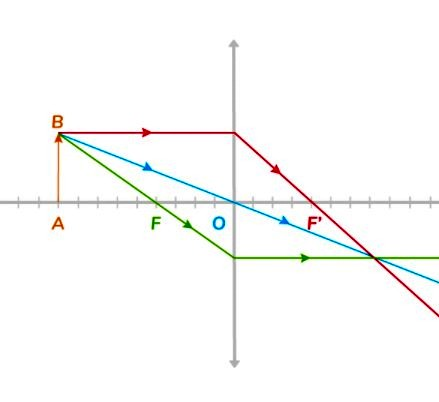
\includegraphics[width=.95\linewidth]{imgs/p6/constrct4.jpg}  
\end{subfigure}
\begin{subfigure}{.18\textwidth}
  \centering
  % fifth  image
  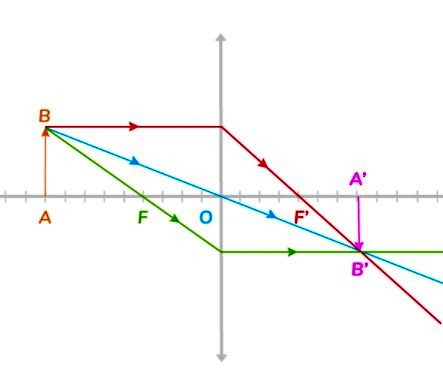
\includegraphics[width=.95\linewidth]{imgs/p6/constrct5.jpg}  
\end{subfigure}
\caption{Les étapes de la construction d'une image à travers une lentille convergente.}
\end{figure}
\newpage
\begin{eg}
\begin{center}
    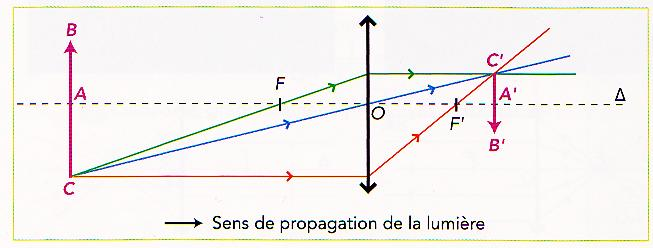
\includegraphics[width=\textwidth]{imgs/p6/imageconstruct.jpg}    
\end{center}
\end{eg}

\subsection{Caractérisation d'une image formée}

L'image qui se forme, à travers un système optique, peut être soit \textbf{réelle}, soit \textbf{virtuelle}. 

\begin{defn}{Images et objets réels \& virtuels}

\begin{itemize}
    \item Si l’\textbf{image} se forme du côté « image », c’est-à-dire « \textbf{après} » la lentille, elle est appelée \textbf{réelle}. 
    \item Si l’\textbf{image} se forme du côté « objet », c’est-à-dire « \textbf{avant} » la lentille, elle est appelée \textbf{virtuelle}. 
    \item Si l’\textbf{objet} est situé du côté « objet », c’est-à-dire « avant » la lentille, il est \textbf{réel}. 
    \item Si l’\textbf{objet} est situé du côté « image », c’est-à-dire « après » la lentille, il est \textbf{virtuel}. 
\end{itemize}
Les sens \textit{avant} et \textit{après} sont entendus par rapport au sens de propagation de la lumière, comme mentionné précédemment. 
\end{defn}

\begin{eg}
\begin{center}
    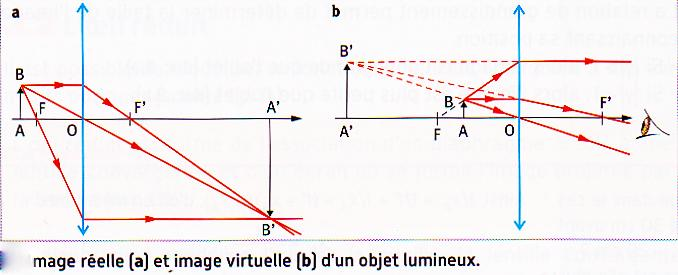
\includegraphics[width=0.6\textwidth]{imgs/p6/imagesvirtuelle.jpg}
\end{center}
\end{eg}

\begin{rmrq}
Il existe une équation, nommé \emph{la relation de conjugaison}, qui permet d'établir un relation mathématique entre la distance objet-centre optique $\overline{AO}$, la distance centre optique-image $\overline{OA'}$, et la distance focale de la lentille $f'$. Voici la relation de conjugaison : 
\[ \dfrac{1}{\overline{OA'}} - \dfrac{1}{\overline{OA}} = \dfrac{1}{\overline{f'}}\]
Vous pouvez vous servir de cette relation pour vérifier les images construites graphiquement. 
\end{rmrq}

\subsection{Grandissement}

\begin{defn}{Grandissement\eng{Magnification}}
\begin{itemize}
    \item Le grandissement est le rapport entre la taille de l’image et l’objet.
    \item Il est utilisé afin de caractériser le changement de taille effectué par le système optique. 
    \item Le grandissement est noté avec le symbole $\gamma$ (gamma). 
    \item C'est une grandeur sans unité. 
    \item Le grandissement est déterminé grâce à l'exprssion : 
    \[ \gamma = \dfrac{\overline{A'B'}}{\overline{AB}} = \dfrac{\overline{OA'}}{\overline{OA}}     \]
\end{itemize}
\end{defn}

Faisons donc quelques remarques d'après les résultats précédents : 
\begin{itemize}
    \item les grandeurs $\overline{A'B'}$ ou $\overline{AB}$ sont des grandeurs orientées, et donc il faut respecter leurs orientations physique en leur attribuant le bon signe $-/+$. 
    \item Le signe de $\gamma$ signifie si l'image est dans le même sens que l'objet ($\gamma>0$) ou renversée ($\gamma<0$).
    \item La norme du grandissement $ \abs{\gamma}$ signifie le facteur de grandissement. 
    \item L'image est plus grande si $ \abs{\gamma}>1 $ et plus petite si $ \abs{\gamma}<1$. 
\end{itemize}

\begin{rmrq}
Afin d’optimiser la qualité d’une imagé formée à travers d’une lentille on exige un ensemble de conditions appelé les \textbf{« conditions de Gauss »} :
\begin{itemize}
    \item Le faisceau doit traverser la lentille au voisinage du centre optique.
    \item Les rayons incidents doivent faire un angle faible avec l'axe optique de la lentille.
\end{itemize}
Sauriez-vous justifier les conditions de Gauss? (Penser à la réfraction de lumière polychromatique en passant par un dioptre séparant deux milieux différents)...
\end{rmrq}

\section{Modèle de la lunette astronomique}
La lunette astronomique a été inventé date d'avant Galilée (n. 1564) et Kepler (n. 1571), mais ils sont responsables, tous les deux, en partie de sa mise au point au cours du XVI et XVII siècles. Pour contexte, le microscope moderne a été inventé par Van Leeuwenhoek au cours du XVII siècle. 

Dans un certain sens une lunette astronomique et un microscope sont très semblables : les deux ont pour fonction d'agrandir l'image des objets très petits. La différence entre les deux est la distance entre l'objet et l'appareil : les objets vus par un microscope sont très très proches (et très petits), tandis que les objets vus par une lunette astronomiques sont à une très grande distance (considérés comme à l'infini) et sont, en réalité, très grands. Leur taille petite est en fait une \textit{taille apparente}. Le fait donc, que ces objets soient très distant a une conséquence fondamentale : le \textbf{rayons provenant de ces objets, venant de l'infini, sont parallèles entres eux}. 

Dans les deux cas, l'image créée et projetée par l'appareil doit être projetée à l'infini (pour que nos yeux n'aient pas à accommoder, et donc réduire la fatigue).  

\subsection{Système afocal}
La lunette astronomique est un \textbf{instrument optique afocal}, c'est-à-dire c'est un instrument optique \textbf{n'ayant pas de foyer}. Autrement dit l'instrument ne fait ni converger ni diverge les rayons lumineux qui y entrent. 

\textbf{Il s'agit d'un système formant une image à l'infini, à partir d'un objet situé à l'infini.} 

\subsection{Composition de la lunette astronomique}

Le modèle le plus simple de la lunette astronomique comporte deux lentilles minces : 
\begin{itemize}
    \item Une lentille mince $\mathcal{L}_1$, appelé l'\textbf{objectif} (car elle est du coté objet), avec la distance focale $f_1'$, dont le rôle est de recevoir la lumière venant de l'objet (ici objet céleste). 
    \item Une lentille mince $\mathcal{L}_2$, appelé l'\textbf{oculaire} (car elle est du coté \oe il), avec la distance focale $f_2'$, dont le rôle est de projeter l'image à l'infini, dans l'\oe il de l'observateur. 
\end{itemize}


Dans un premier temps, les rayons venant de l'infini convergent sur le foyer image d'un objectif, et donc la lumière entrant dans l'objectif converge sur son plan focal, situé à $f_1'$. Il y a donc une \textbf{image intermédiaire} qui se forme, à l'intérieur de la lunette à $f_1'$. 

De l'autre côté le rôle de l'oculaire est de projeter les images venant de l'objectif, à l'infini (pour que l'\oe il n'ait pas à accommoder, pour éviter la fatigue). Pour qu'une image soit projetée à l'infini, il faut que l'objet soit situé sur le foyer objet de la lentille mince à $f_2'$ du centre optique de l'oculaire. 

\begin{figure}[H]
\centering
\begin{subfigure}{.47\textwidth}
  \centering
  % include first image
  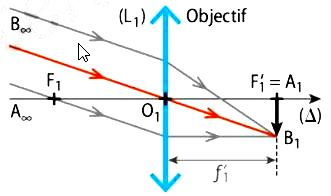
\includegraphics[width=.95\linewidth]{imgs/p6/objectif.jpg}
  \caption{Rôle de l'objectif. }
\end{subfigure}
\begin{subfigure}{.47\textwidth}
  \centering
  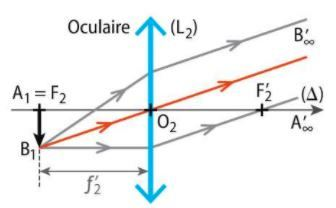
\includegraphics[width=.95\linewidth]{imgs/p6/oculaire.jpg}  
  \caption{Rôle de l'oculaire. }    
\end{subfigure}
\caption{Les composantes d'une lunette astronomique afocale.  } 
\end{figure}

L'\textbf{image formée par l'objectif, est l'objet pour l'oculaire}. La seule chose qui reste à faire est donc de positionner les deux lentilles tel que l'image intermédiaire soit bien placée sur le foyer objet de l'oculaire. \textbf{Il faut donc le foyer image de l'objectif $F_1'$ et le foyer objet de l'oculaire $F_2$ soit confondus} comme dans le figure \ref{fig:lunette}, ci-après. La distance $O_1O_2 = f'_1 + f'_2$.

\begin{figure}[H]
    \centering
    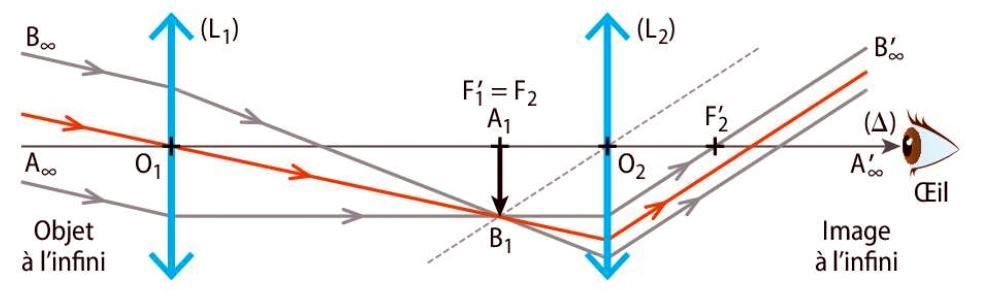
\includegraphics[width=.95\linewidth]{imgs/p6/lunette.jpg}
    \caption{Schéma d'une lunette astronomique}
    \label{fig:lunette}
\end{figure}

\begin{exo}
Tracer le chemin des rayons lumineux pour une lunette astronomique avec $f'_1 = 5\,cm$ et $f'_2 = 2\,cm$

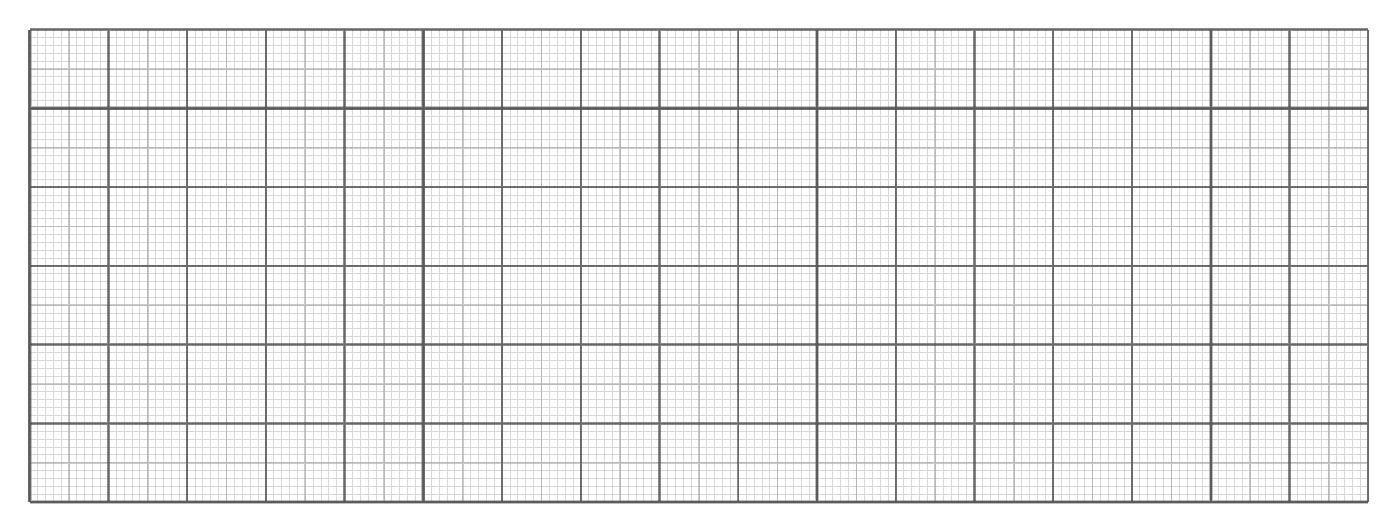
\begin{tikzpicture}[x=1cm, y=1cm, semitransparent]
\draw[step=1mm, line width=0.1mm, black!30!white] (0,0) grid (17,6);
\draw[step=5mm, line width=0.2mm, black!40!white] (0,0) grid (17,6);
\draw[step=5cm, line width=0.5mm, black!50!white] (0,0) grid (17,6);
\draw[step=1cm, line width=0.3mm, black!90!white] (0,0) grid (17,6);
\end{tikzpicture}
\end{exo}

\section{Grossissement}
On se rappelle que l'on caractérise un système optique, comme une loupe ou n'importe quel autre appareil qui sert à augmenter la taille d'un objet, par son \textbf{grandissement} (c.f. . Cela n'est pas possible avec un système afocal car l'objet est à l'infini, et très grand. Nous caractérisons donc, cette amplification, par une nouvelle grandeur semblable qui s'appelle le \textbf{grossissement}. 

\begin{defn}{Grossissement}
\begin{itemize}
    \item Le grossissement $G$ d'un système optique est défini comme le quotient de l'angle $\alpha'$ sous lequel on voit un objet à l'infini à travers l'instrument, par l'angle $\alpha$ sous lequel on voit l'objet à l'\oe il nu. \item Le grossissement est donné par la formule : 
    \[  G = \frac{\alpha'}{\alpha}      \]
\end{itemize}
\end{defn}

\begin{figure}[H]
    \centering
    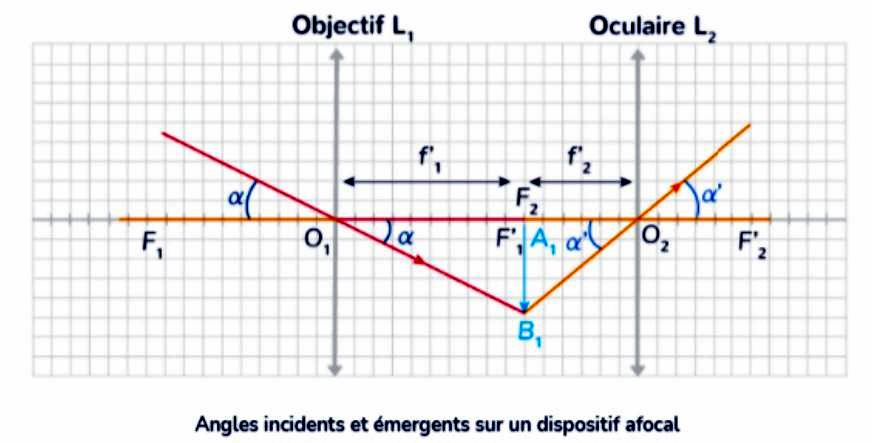
\includegraphics[width=.95\linewidth]{imgs/p6/gros1.jpg}
\end{figure}

Considérons maintenant les triangles $O_1A_1B_1$ et $O_2A_1B_1$, qui partagent le côté $A_1B_1$. $\tan \alpha = \dfrac{A_1B_1}{f_1'}$ et $\tan \alpha' = \dfrac{A_1B_1}{f_2'}$.

D'après l'\textbf{approximation des petits angles} ($\theta \approx \tan \theta$ valables tant que $\tehta<10\degree$) : 

\[
    G &= \dfrac{\alpha'}{\alpha} = \dfrac{\tan\alpha'}{\tan\alpha}  = \dfrac{\frac{A_1B_1}{f_2'}}{\frac{A_1B_1}{f_1'}} = \dfrac{f_1'}{f_2'}
\]

Et donc, on peut déterminer le grossissement d'une lunette astronomique en comparant les distances focales de l'objectif et de l'oculaire : $G = \dfrac{f_1'}{f_2'} = \dfrac{C_2}{C_1} $


\end{document}